\documentclass[14pt]{extbook}
\usepackage{multicol, enumerate, enumitem, hyperref, color, soul, setspace, parskip, fancyhdr} %General Packages
\usepackage{amssymb, amsthm, amsmath, bbm, latexsym, units, mathtools} %Math Packages
\everymath{\displaystyle} %All math in Display Style
% Packages with additional options
\usepackage[headsep=0.5cm,headheight=12pt, left=1 in,right= 1 in,top= 1 in,bottom= 1 in]{geometry}
\usepackage[usenames,dvipsnames]{xcolor}
\usepackage{dashrule}  % Package to use the command below to create lines between items
\newcommand{\litem}[1]{\item#1\hspace*{-1cm}\rule{\textwidth}{0.4pt}}
\pagestyle{fancy}
\lhead{Progress Quiz 4}
\chead{}
\rhead{Version A}
\lfoot{4378-7085}
\cfoot{}
\rfoot{Fall 2020}
\begin{document}

\begin{enumerate}
\litem{
Solve the radical equation below. Then, choose the interval(s) that the solution(s) belongs to.\[ \sqrt{16 x^2 - 56} - \sqrt{4 x} = 0 \]\begin{enumerate}[label=\Alph*.]
\item \( x \in [1.82,2.2] \)
\item \( x \in [-1.84,-1.3] \)
\item \( \text{All solutions lead to invalid or complex values in the equation.} \)
\item \( x_1 \in [-1.84, -1.3] \text{ and } x_2 \in [-1,4] \)
\item \( x_1 \in [1.56, 1.83] \text{ and } x_2 \in [-1,4] \)

\end{enumerate} }
\litem{
Solve the radical equation below. Then, choose the interval(s) that the solution(s) belongs to.\[ \sqrt{5 x + 6} - \sqrt{6 x + 6} = 0 \]\begin{enumerate}[label=\Alph*.]
\item \( x \in [-1,3] \)
\item \( \text{All solutions lead to invalid or complex values in the equation.} \)
\item \( x_1 \in [-2.2, -0.2] \text{ and } x_2 \in [-0.53,1.74] \)
\item \( x_1 \in [-2.2, -0.2] \text{ and } x_2 \in [-1.1,-0.2] \)
\item \( x \in [7,15] \)

\end{enumerate} }
\litem{
Choose the graph of the equation below.\[ f(x) = - \sqrt[3]{x + 12} - 7 \]\begin{enumerate}[label=\Alph*.]
\begin{multicols}{2}\item 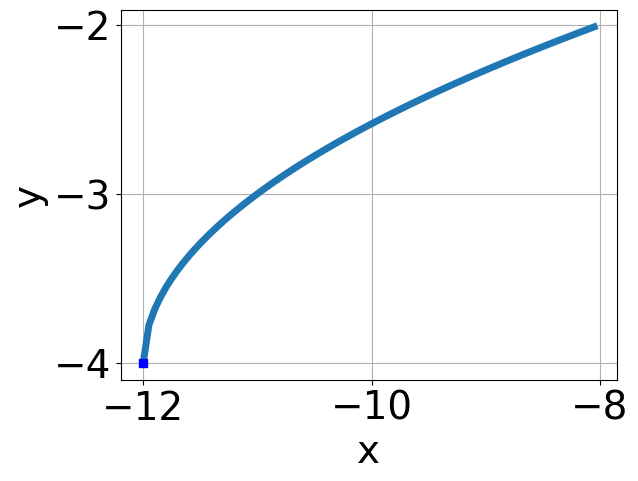
\includegraphics[width = 0.3\textwidth]{../Figures/radicalEquationToGraphCopyAA.png}\item 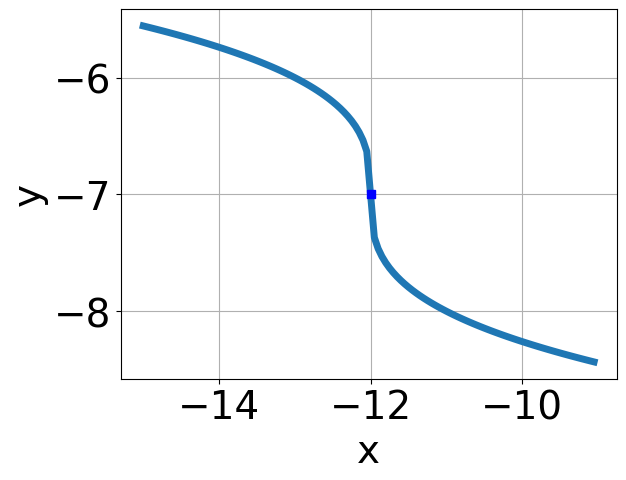
\includegraphics[width = 0.3\textwidth]{../Figures/radicalEquationToGraphCopyBA.png}\item 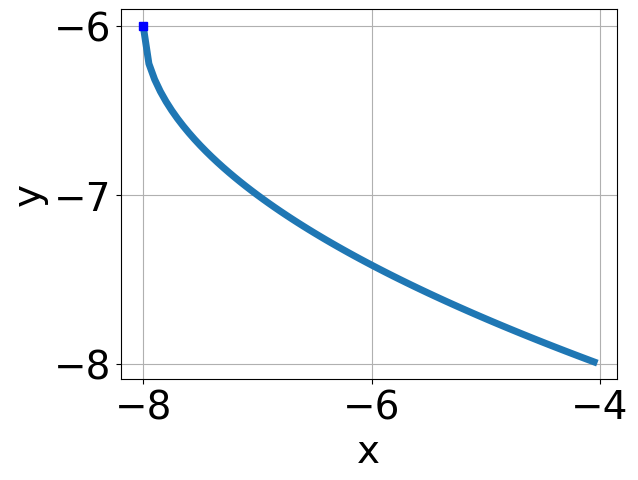
\includegraphics[width = 0.3\textwidth]{../Figures/radicalEquationToGraphCopyCA.png}\item 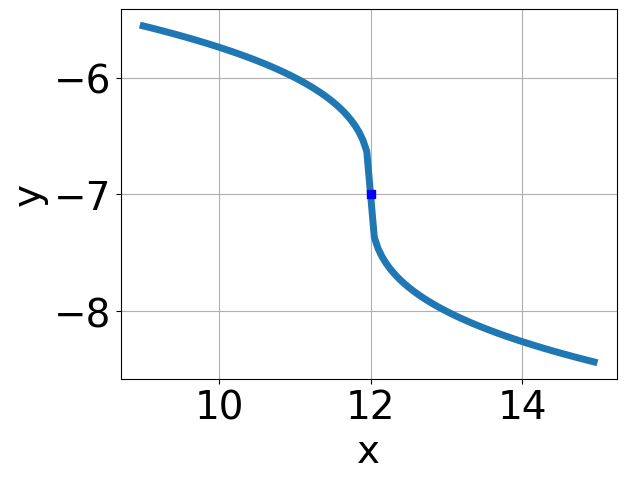
\includegraphics[width = 0.3\textwidth]{../Figures/radicalEquationToGraphCopyDA.png}\end{multicols}\item None of the above.
\end{enumerate} }
\litem{
What is the domain of the function below?\[ f(x) = \sqrt[5]{4 x - 9} \]\begin{enumerate}[label=\Alph*.]
\item \( \text{The domain is } [a, \infty), \text{   where } a \in [-1.7, 1.3] \)
\item \( \text{The domain is } (-\infty, a], \text{   where } a \in [-2.8, 2.2] \)
\item \( \text{The domain is } (-\infty, a], \text{   where } a \in [1.1, 5.1] \)
\item \( \text{The domain is } [a, \infty), \text{   where } a \in [0.6, 3.6] \)
\item \( (-\infty, \infty) \)

\end{enumerate} }
\litem{
Solve the radical equation below. Then, choose the interval(s) that the solution(s) belongs to.\[ \sqrt{-18 x^2 - 14} - \sqrt{48 x} = 0 \]\begin{enumerate}[label=\Alph*.]
\item \( x \in [-0.9,0.4] \)
\item \( x_1 \in [-4.8, -1.2] \text{ and } x_2 \in [-0.52,-0.21] \)
\item \( x_1 \in [1.4, 2.6] \text{ and } x_2 \in [0.33,0.41] \)
\item \( \text{All solutions lead to invalid or complex values in the equation.} \)
\item \( x \in [-4.8,-1.2] \)

\end{enumerate} }
\litem{
Choose the equation of the function graphed below.
\begin{center}
    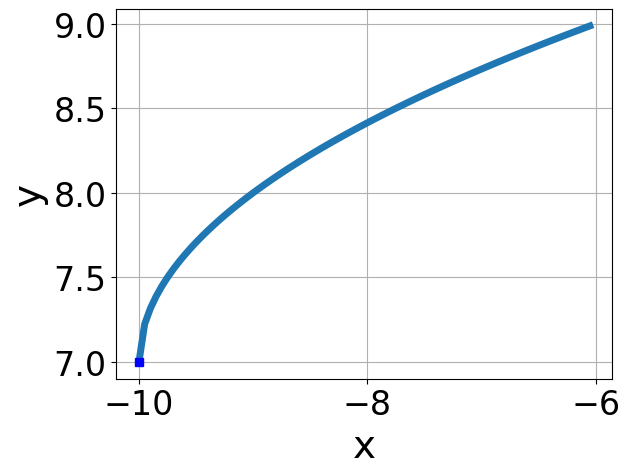
\includegraphics[width=0.5\textwidth]{../Figures/radicalGraphToEquationCopyA.png}
\end{center}
\begin{enumerate}[label=\Alph*.]
\item \( f(x) = - \sqrt[3]{x + 8} - 4 \)
\item \( f(x) = \sqrt[3]{x + 8} - 4 \)
\item \( f(x) = \sqrt[3]{x - 8} - 4 \)
\item \( f(x) = - \sqrt[3]{x - 8} - 4 \)
\item \( \text{None of the above} \)

\end{enumerate} }
\litem{
Choose the graph of the equation below.\[ f(x) = - \sqrt{x + 10} + 3 \]\begin{enumerate}[label=\Alph*.]
\begin{multicols}{2}\item 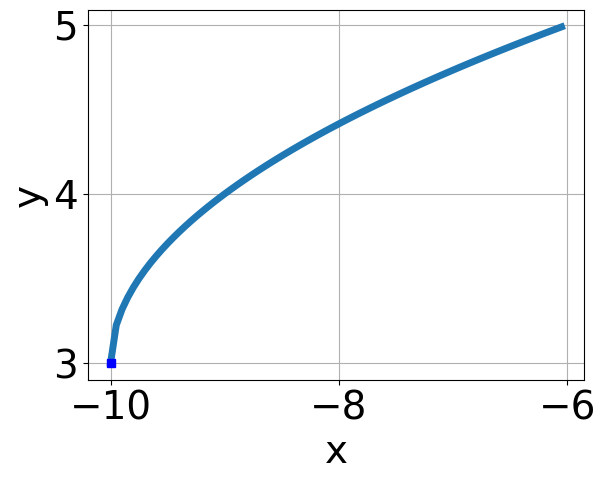
\includegraphics[width = 0.3\textwidth]{../Figures/radicalEquationToGraphAA.png}\item 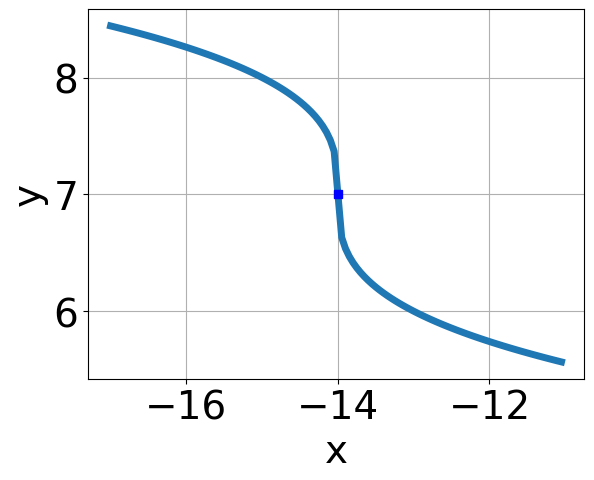
\includegraphics[width = 0.3\textwidth]{../Figures/radicalEquationToGraphBA.png}\item 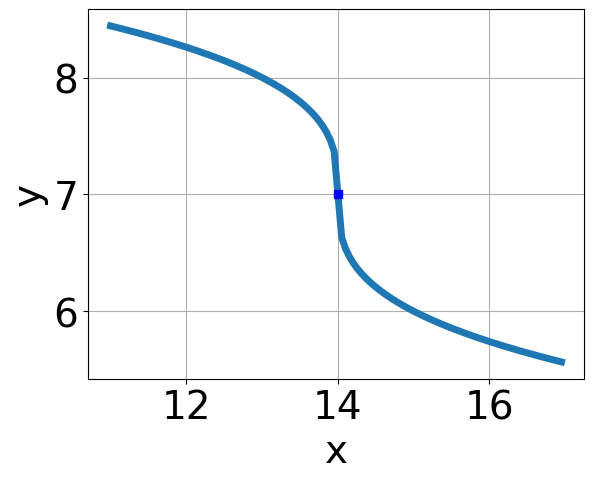
\includegraphics[width = 0.3\textwidth]{../Figures/radicalEquationToGraphCA.png}\item 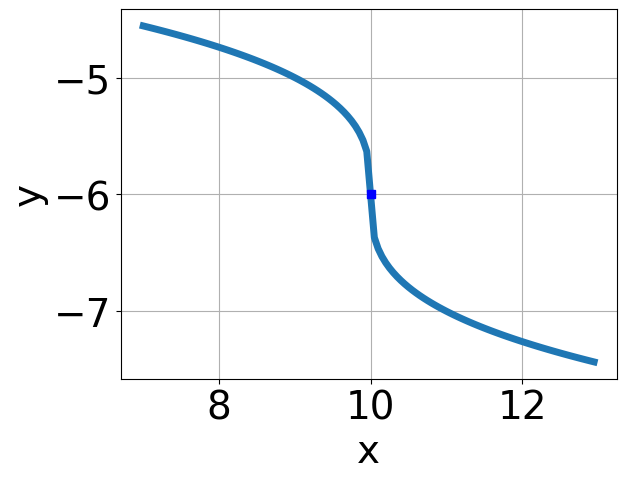
\includegraphics[width = 0.3\textwidth]{../Figures/radicalEquationToGraphDA.png}\end{multicols}\item None of the above.
\end{enumerate} }
\litem{
Solve the radical equation below. Then, choose the interval(s) that the solution(s) belongs to.\[ \sqrt{-2 x + 8} - \sqrt{-9 x + 6} = 0 \]\begin{enumerate}[label=\Alph*.]
\item \( x \in [-2.42,-0.67] \)
\item \( \text{All solutions lead to invalid or complex values in the equation.} \)
\item \( x_1 \in [0.59, 0.91] \text{ and } x_2 \in [3,8] \)
\item \( x \in [-1.94,0.35] \)
\item \( x_1 \in [-1.94, 0.35] \text{ and } x_2 \in [3,8] \)

\end{enumerate} }
\litem{
What is the domain of the function below?\[ f(x) = \sqrt[5]{-3 x - 5} \]\begin{enumerate}[label=\Alph*.]
\item \( (-\infty, \infty) \)
\item \( \text{The domain is } (-\infty, a], \text{   where } a \in [-1.24, -0.52] \)
\item \( \text{The domain is } (-\infty, a], \text{   where } a \in [-3.69, -1.1] \)
\item \( \text{The domain is } [a, \infty), \text{   where } a \in [-1.96, -0.66] \)
\item \( \text{The domain is } [a, \infty), \text{   where } a \in [-0.7, -0.17] \)

\end{enumerate} }
\litem{
Choose the equation of the function graphed below.
\begin{center}
    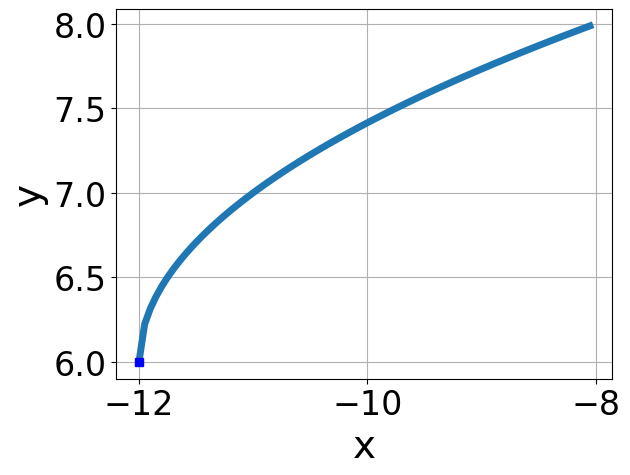
\includegraphics[width=0.5\textwidth]{../Figures/radicalGraphToEquationA.png}
\end{center}
\begin{enumerate}[label=\Alph*.]
\item \( f(x) = \sqrt{x - 10} - 7 \)
\item \( f(x) = - \sqrt{x - 10} - 7 \)
\item \( f(x) = - \sqrt{x + 10} - 7 \)
\item \( f(x) = \sqrt{x + 10} - 7 \)
\item \( \text{None of the above} \)

\end{enumerate} }
\end{enumerate}

\end{document}